

\begin{itemize}
	\item \textit{CalendarMaagement}, sends requests to update the calendar. Besides that it provide invites to be sent on to the \textit{ShareSubsystem}. 
	\item \textit{ShareSubsystem} sends request of wathever data the google client wants to the \textit{CalendarManagement}.
	\item \textit{SyncSubsystem} The \textit{SyncSubsystem} the decides wich storage sould be used in terms of the network connection at the time it gets a request from \textit{CalendarManagement}.
\end{itemize}

\begin{figure}[ht!]
\centering
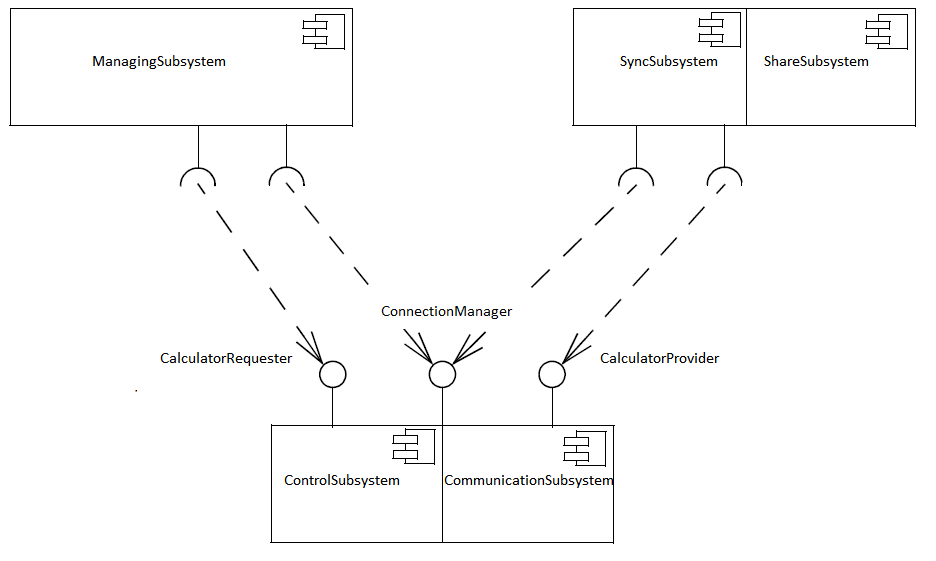
\includegraphics[width=160mm]{UMLComponentService.png}
\caption{Subsystem decomposition with services (UML Component diagram) \label{overflow}}
\end{figure}
